% !TEX program = lualatex
\documentclass{article}
\usepackage{fontspec}
\usepackage{luatexja-fontspec}
\usepackage{luatexja-ruby} % ルビを使用する場合に必要
\usepackage{graphicx}
\usepackage{listings}
%\usepackage{xcolor}

% フォントの設定
%\setmainfont{Noto Serif JP}    % 通常の明朝体
%\setsansfont{Noto Sans JP}     % 通常のゴシック体
%\setmonofont{Noto Sans Mono JP} % 等幅フォント
%\setmainjfont{Noto Serif JP}   % 日本語の明朝体
%\setsansjfont{Noto Sans JP}    % 日本語のゴシック体
%\setmonojfont{Noto Sans Mono JP} % 日本語の等幅フォント

% 図の参照パス
\graphicspath{{./01_code/output/}}

% コードのスタイル設定
\lstset{
  basicstyle=\ttfamily\small, % フォントのサイズとスタイル
  %keywordstyle=\color{blue},  % キーワードの色
  %commentstyle=\color{gray},  % コメントの色
  %stringstyle=\color{red},    % 文字列の色
  numbers=left,               % 行番号を左側に表示
  %numberstyle=\tiny\color{gray}, % 行番号のスタイル
  breaklines=true,            % 長い行を折り返す
	frame=single,               % コードブロックに枠をつける
}

\begin{document}

% タイトル
\title{ミクロデータサイエンス\\Problemset1}
\author{2125178\\廣江友哉}
\date{\today}
\maketitle


% 段落
\section{サイコロと一様分布}

\subsection{分布の形}

どの実現値においても同じ確率 1/6 を取る長方形のような形の分布になる。

\subsection{コードの実行結果の考察}

\begin{lstlisting}[]
	calculate_scores <- function(m, n, seed_num) {
		set.seed(seed_num)
		score <- replicate(n, sum(roll_dice(m)))
		df_score <- dplyr::tibble(score)
		plot_scores(df_score)
	}

\end{lstlisting}

	\begin{center}
		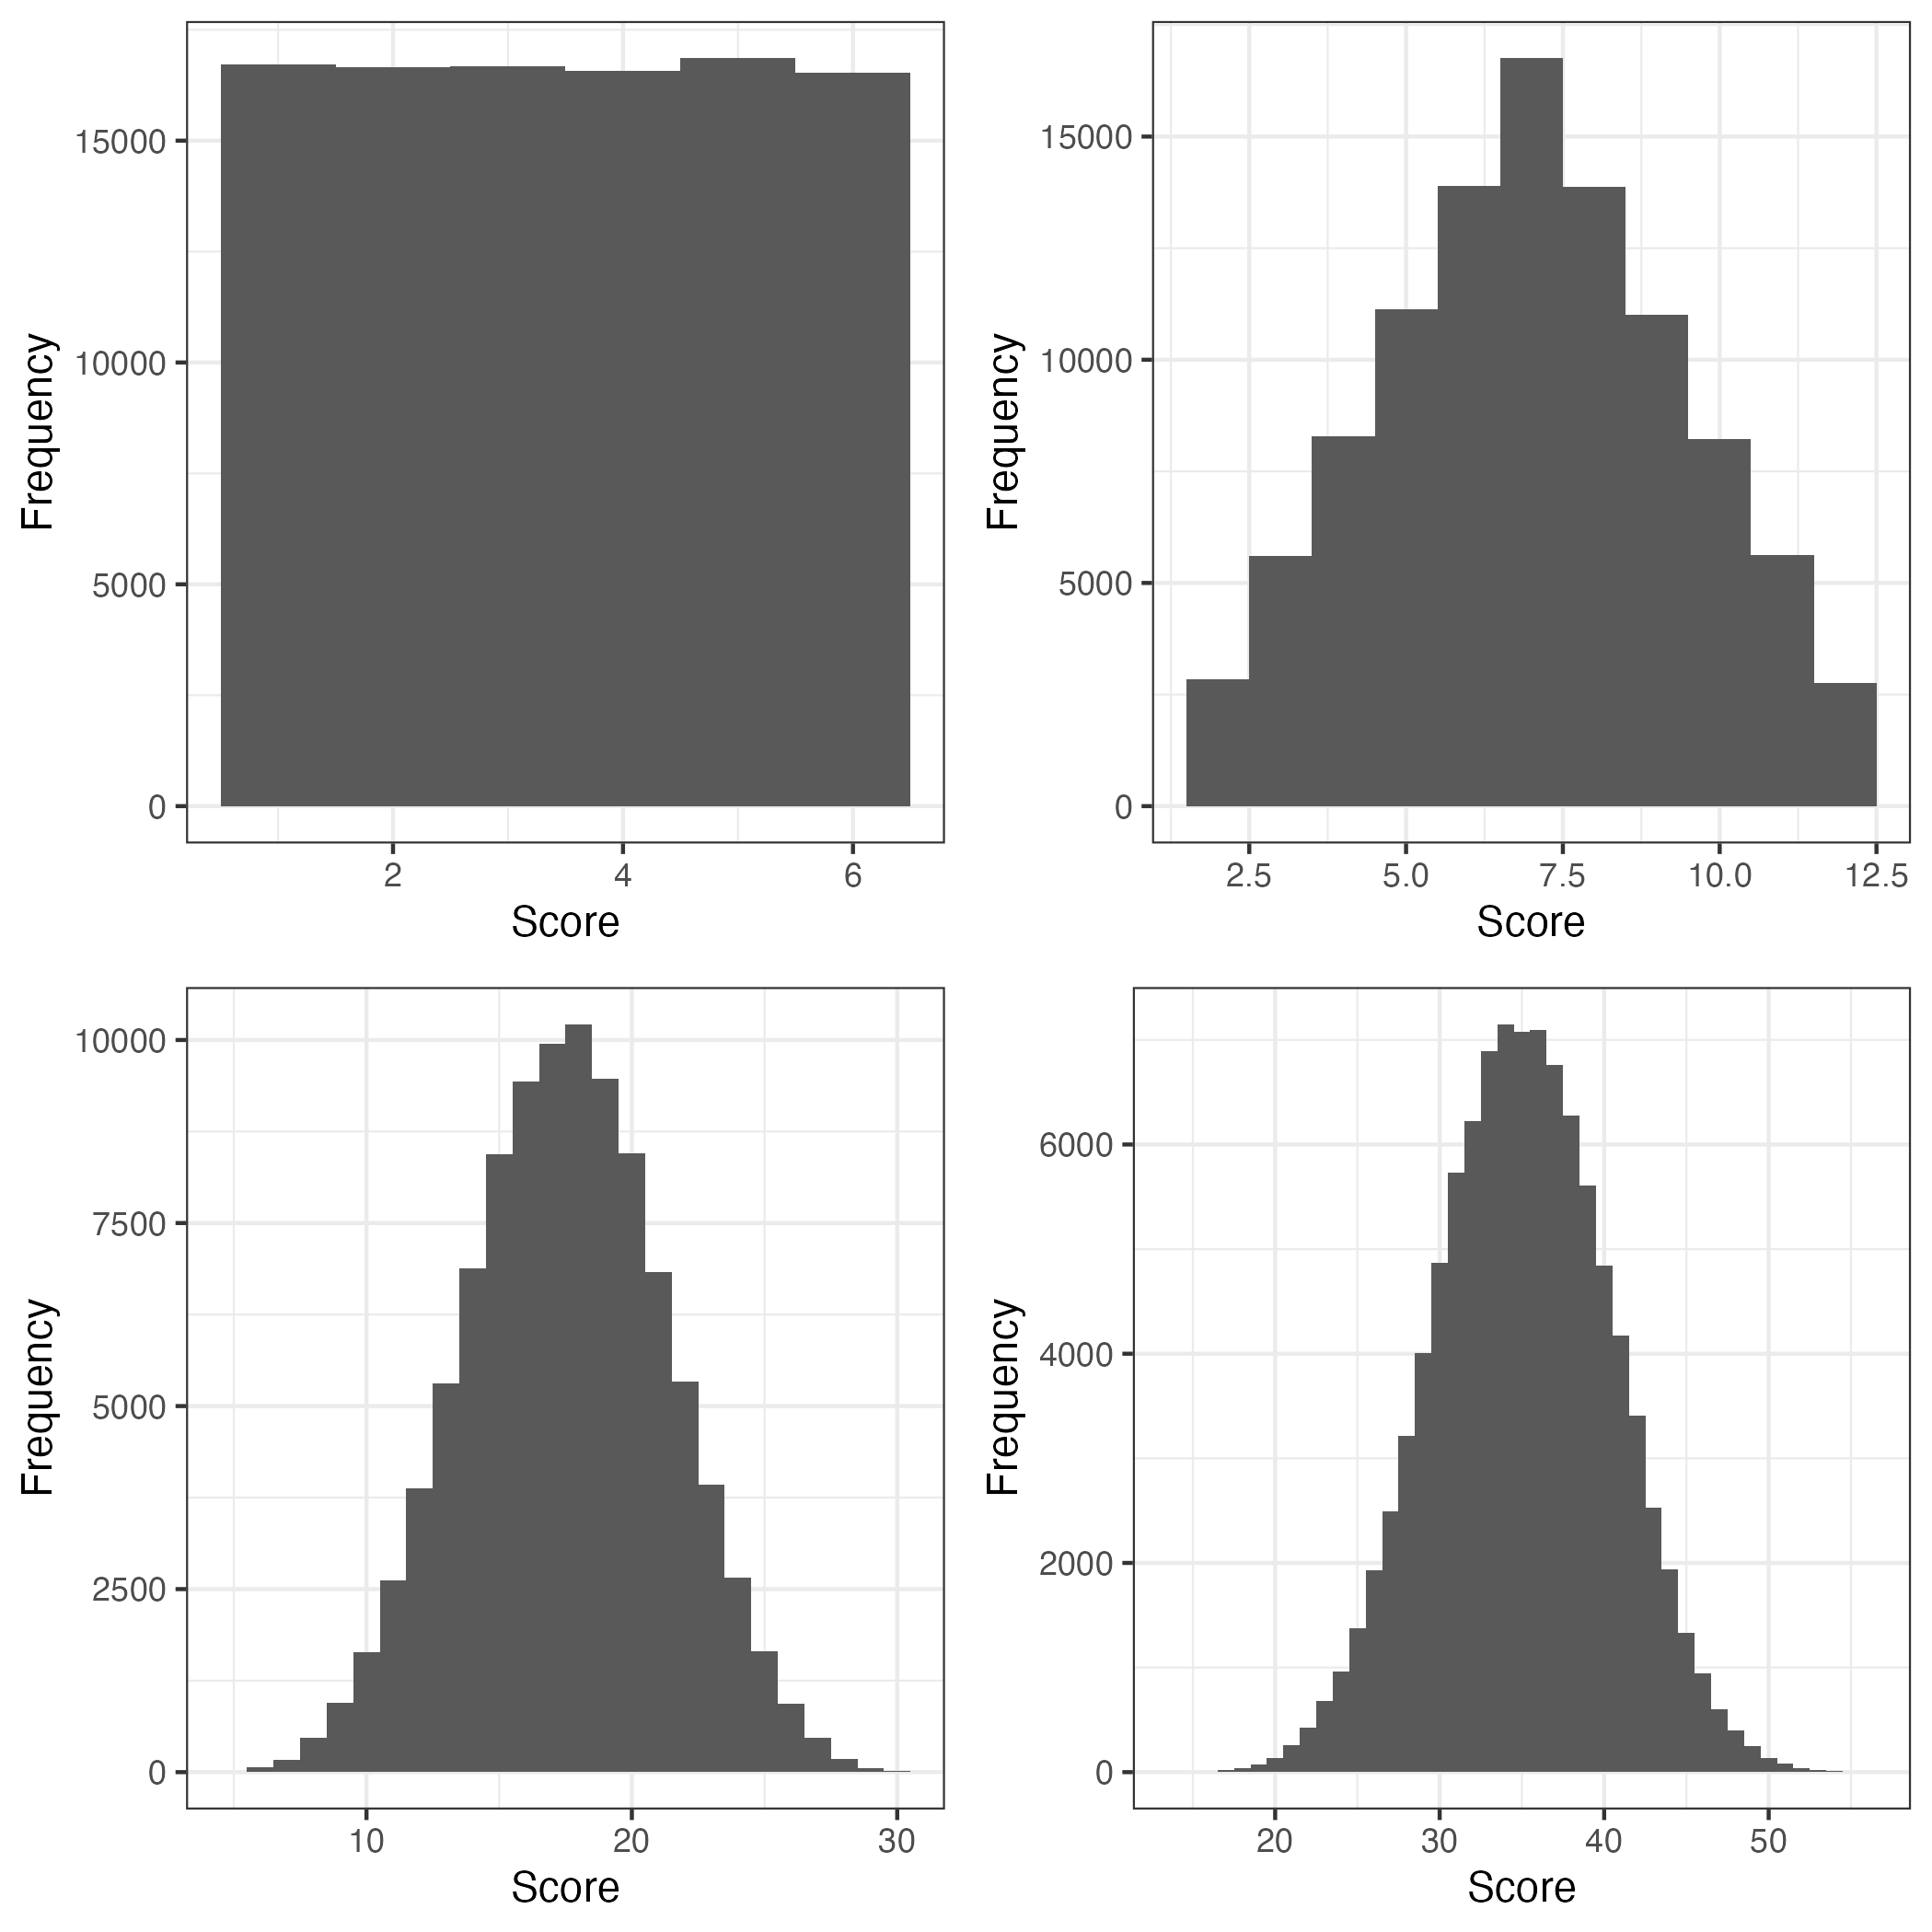
\includegraphics[width=0.7\textwidth]{1-2_plot.png}
	\end{center}

上図は、左上から順に、m = 1,2,5,10 の時の分布である。 
m = 1 の時は 1-1 で回答したように一様分布に従っている。\\
m = 2 から m = 10 にかけて少しずつ正規分布に近似していくのが見て取れる。\\
ここから、一様分布に従う確率変数の和は繰り返すと正規分布に近似することが考察できる。

\subsection{確率分布の和の分布のシミュレーションadv}

\subsection{標本平均の分散の変化}
	\begin{center}
		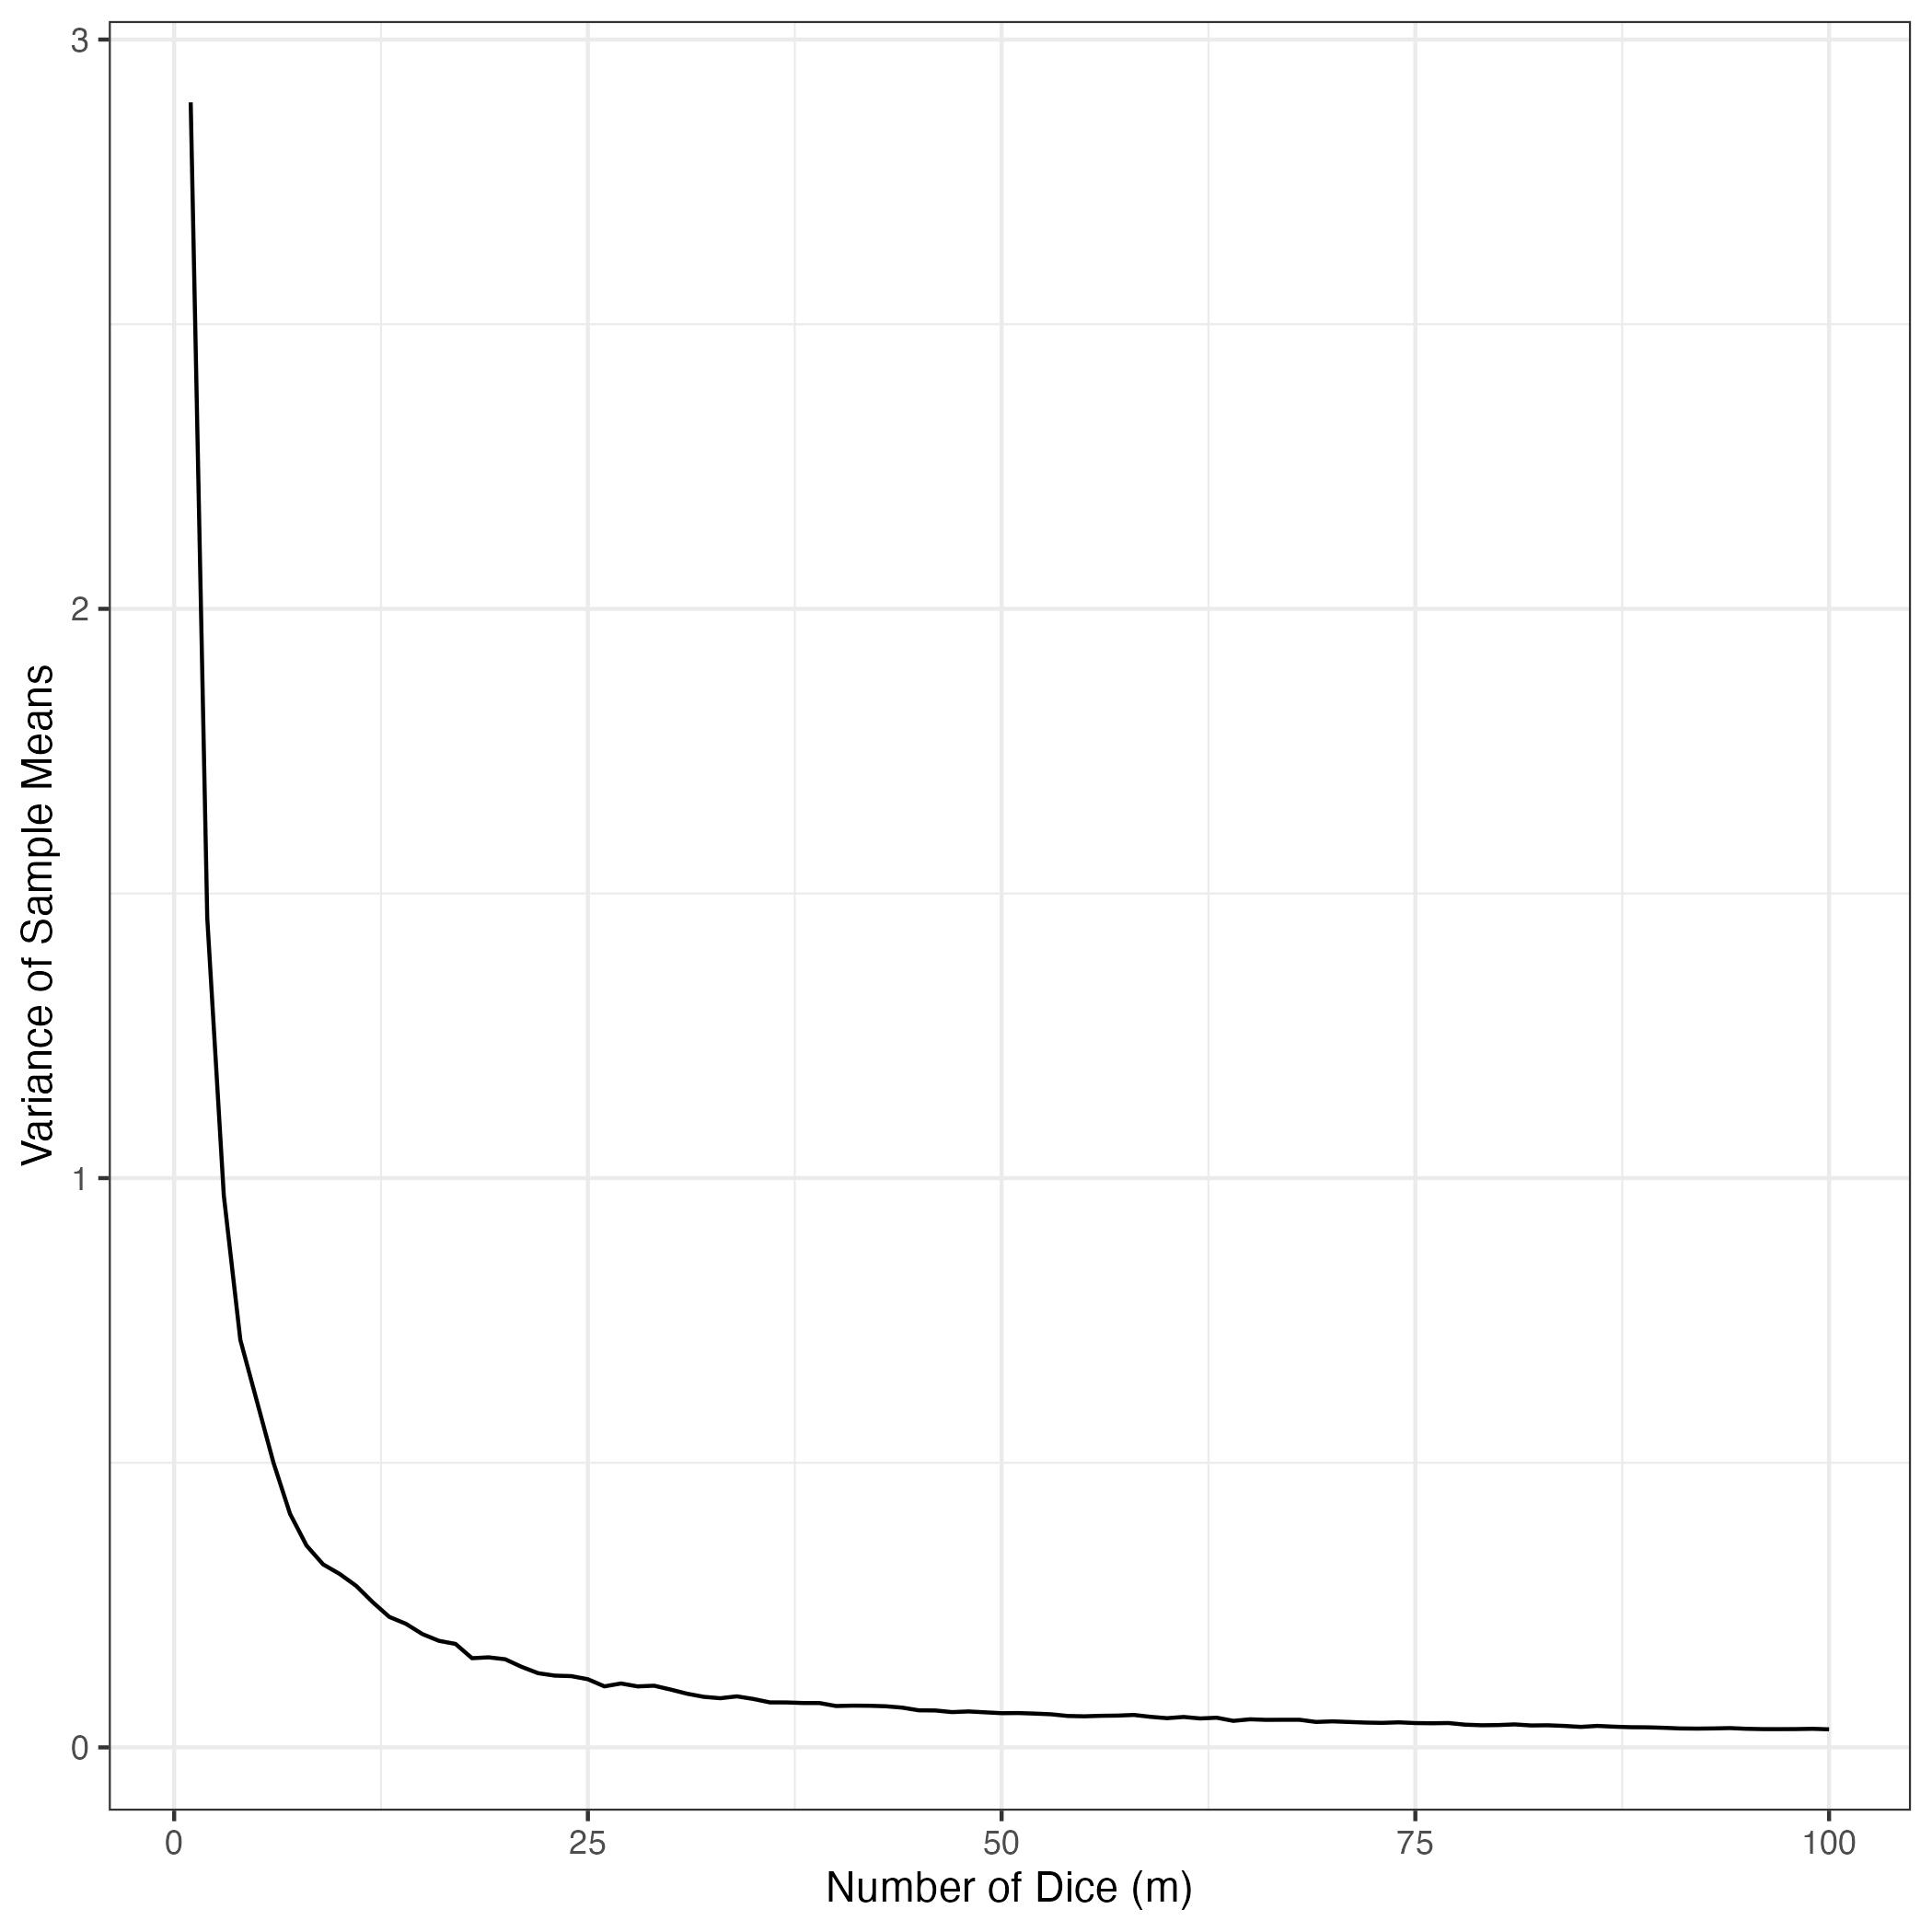
\includegraphics[width=0.7\textwidth]{1-4_plot.png}
	\end{center}

サイコロの数が増える、つまり、和をとる確率変数の数が増えるほど
標本平均の分散は指数関数的に減少していく傾向になることがわかる。

\section{指数分布と故障}
\subsection{タブレットの導入(学校側)}
\subsubsection{指数分布のパラメータλ}

「サーバの故障回数は、1 年間に平均 2.5 回の指数分布に従う」ので、以下のような式を導ける。

\[ E[t] = \frac{1}{\lambda} = 2.5 \]

したがって、パラメータ\lambda は 2.5 となる。

\subsubsection{1年間で発生する期待コスト}






\end{document}
